\chapter{Resultados y análisis}
En esta capítulo se va a mostrar y analizar los resultados de realizar la implementación de los algoritmos criptográficos RC5 y TEA.
Primero se dan resultados y análisis individuales, para posteriomente realizar el análisis comparativo.

Las síntesis e implementaciones se llevaron a cabo haciendo uso de la herramienta de desarrollo \textit{Vivado Design Suite} de \textit{Xillinx} bajo la licencia gratuita \textit{WEBPack}. Se hizo utilizó como objetivo de implementación la tarjeta xc7k70tfbv676-1 de la familia de FPGAs \textit{Kintex-7}. En la Tabla \ref{tabRecursosFPGA} se muestran todos los recursos disponibles de la misma. 

\begin{table}[htbp]
  \centering
  \caption{Recursos disponible para el FPGA Kintex-7 xc7k70tfbv676-1 de Xillinx.}
    \begin{tabular}{lr}
    \toprule
    Componente & Cantidad Disponible\\
    \midrule
	Slices & 10250\\
	Slice LUTs & 41000\\
	Slice Registers & 82000\\
	Block RAM & 135\\
	DSPs & 240\\
	I/O ports & 300\\
    \bottomrule
    \end{tabular}%
  \label{tabRecursosFPGA}%
\end{table}%

Para poder obtener las métricas que se analizan se utilizaron los reportes de temporización y utilización que la herramienta ofrece al finalizar el proceso de implementación. Se guardaron estos archivos después de cada sintesís e implementación y se utilizó un \textit{script} de Python para extraer los datos deseados y escribirlos a un archivo CSV (\textit{Comma Separated Values}) para poder abrir el mismo haciendo uso de \textit{Excel} para graficar las diferentes métricas haciendo uso de tablas pivote para un análisis más eficiente.


Cabe aclarar que aunque en un principio no se iba a tomar en cuenta el análisis de temporización, específicamente la frecuencia máxima de reloj, la misma fue agregada a la lista de métricas a analizar debido a que en la implementación realizada la frecuencia máxima de reloj afecta directamente el tiempo de procesamiento para cifrar y descifrar datos y por tanto es una métrica muy importante a analizar. Agregado a esto se puede destacar el hecho de que igualmente a causa de la implementación el variar la cantidad de rondas que cifran o descifran los datos no afectan de ninguna manera la cantidad de recursos del FPGA y solo afectan el tiempo de procesamiento total de cifrado o descifrado.


Otro aspecto importante es que se asumió que los módulos \textit{top} de los algoritmos son módulos que serán parte de un dispositivo más grande (por ejemplo un procesador) y por tanto que ese dispositivo hará uso de tanto los módulos de cifrado y descifrado, así los módulos serán sintetizados e implementados simúltaneamente para cada algoritmo, ya que el análisis de ambos módulos tendrá más valor que el de los módulos por separado. Particularmente para el algoritmo RC5 se hizo que los módulos de cifrado y descifrado compartan el módulo que se encarga de la expansión de llave (\textit{keyExpander} en las Figuras \ref{figCipherBlockDiagram} y \ref{figDecipherBlockDiagram}) esto con la finalidad de consumir la menor cantidad de recursos y hacer lo más óptimo posible el diseño.


Un problema al que se enfrentó al implementar los algoritmos en el FPGA es que la cantidad de salidas y entradas del diseño era muy grande para que el mismo fuera implementable en el FPGA. La solución a esto corresponde a un módulo para serializar y deserializar las entradas y salidas pero el mismo no fue implementado ya que no era uno de los objetivos del proyecto, además de que se consideró innecesario ya que, como se indicó anteriormente, estos algoritmos formarían parte de un dispositivo más grande que ya contará con este módulo. Así para poder implementar el diseño simplemente se pusieron dos puertos, uno de entrada y otro de salida, ambos del tamaño de la palabra y las señales de control de los módulos.

\section{Resultados y análisis del algoritmo TEA} \label{resultadosAnalisisTEA}
Inicialmente se corroboró que el algoritmo funcionara correctamente, esto se logró comparando los resultados de texto cifrado y descifrado con el código en C que se encuentra en los Listados \ref{lstCipherTEA} y \ref{lstDecipherTEA}\footnote{El código para verificar fue ligeramente diferente al de los listados debido a que se tuvo que ajustar para poder variar el tamaño de palabra.}. La Tabla \ref{tabSimTEA} muestra el resultado de cifrado y descifrado al simular con diferentes tamaños de palabra para 32 rondas de cifrado/descifrado. Además la tabla en la columna \textit{layout} indica un número de figura al cual está ligado la implementación para el tamaño de palabra. Este \textit{layout} corresponde al dado por la herramienta de desarrollo para observar la distribución de recursos en el circuito. Además el camino resaltado en blanco en cada \textit{layout} corresponde al \textit{critical path} de cada implementación.

\begin{table}[htbp]
  \centering
  \caption{Resultados de simulación del TEA para diferentes tamaños de palabra.}
    \begin{tabular}{lrrr}
    \toprule
	\begin{tabular}[c]{@{}l@{}}Tamaño\\de palabra\\(bits)\end{tabular} & Texto plano (hex) & Texto cifrado (hex) & Figura \textit{layout} \\
    \midrule
	8 & 0d8d & aba7 & \ref{fig8_32_layout} \\
	\midrule
	16 & 7b0d998d & 829789bc &  \ref{fig16_32_layout} \\
	\midrule
	32 & 3d45f7a7235fcb21 & f5509056d5db9e6a & \ref{fig32_32_layout} \\
	\midrule
	64 & \begin{tabular}[c]{@{}l@{}}0000000006b97b0d\\0000000046df998d\end{tabular}  & \begin{tabular}[c]{@{}l@{}}0d85f88a9ef595ff\\4810210e9e2a4f5e\end{tabular} & \ref{fig64_32_layout} \\
	\midrule
	128 & \begin{tabular}[c]{@{}l@{}}3ca67c8e15890877\\6dcc3a7b41cb88e6\\9a34483d3b1a68a4\\1235130bf207ee95\end{tabular} & \begin{tabular}[c]{@{}l@{}}c0144f6419ce0203\\dbee17be33c2bf5c\\87b4dc12f9cbe22f\\f2f826efc585fa46\end{tabular} & \ref{fig128_32_layout} \\
    \bottomrule
    \end{tabular}%
  \label{tabSimTEA}%
\end{table}%


\begin{figure}[H]
	\centering
	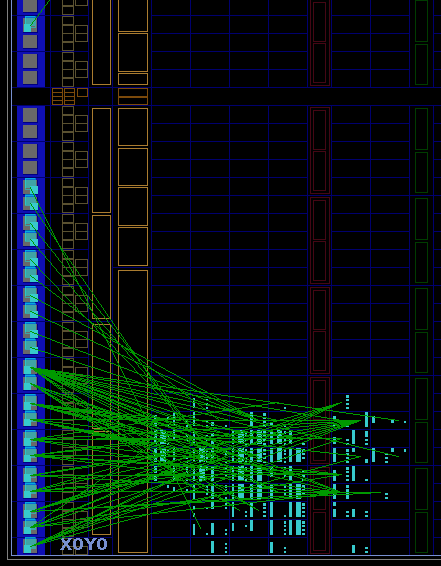
\includegraphics[width=0.9\textwidth]{./images/fig8_32_layout}
	\caption{\textit{Layout} de la implementación del algoritmo TEA de 8 bits de tamaño de palabra y 32 rondas de cifrado/descifrado.}
	\label{fig8_32_layout}
\end{figure}

\begin{figure}[H]
	\centering
	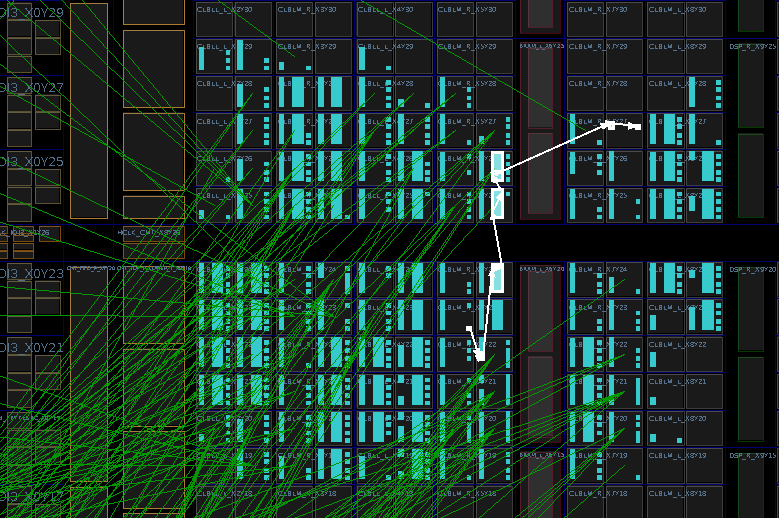
\includegraphics[width=0.9\textwidth]{./images/fig16_32_layout}
	\caption{\textit{Layout} de la implementación del algoritmo TEA de 16 bits de tamaño de palabra y 32 rondas de cifrado/descifrado.}
	\label{fig16_32_layout}
\end{figure}

\begin{figure}[H]
	\centering
	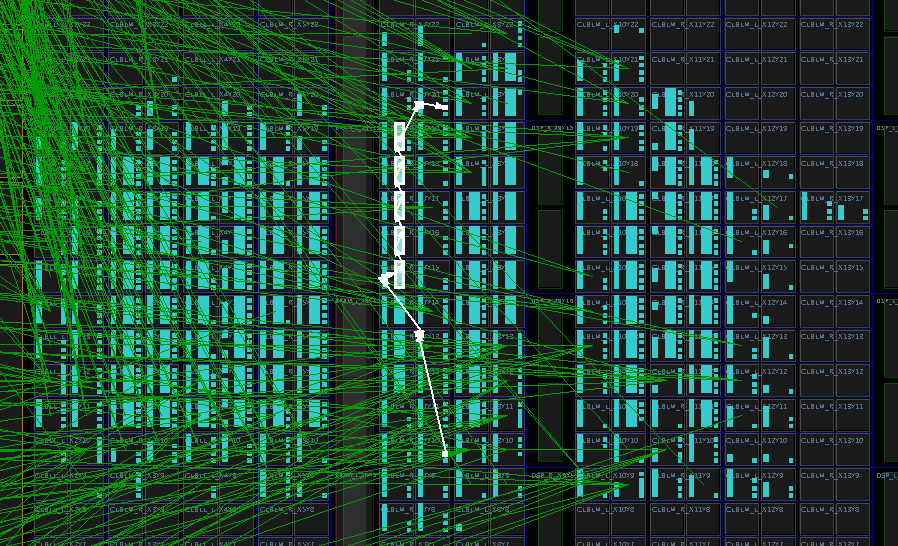
\includegraphics[width=0.9\textwidth]{./images/fig32_32_layout}
	\caption{\textit{Layout} de la implementación del algoritmo TEA de 32 bits de tamaño de palabra y 32 rondas de cifrado/descifrado.}
	\label{fig32_32_layout}
\end{figure}

\begin{figure}[H]
	\centering
	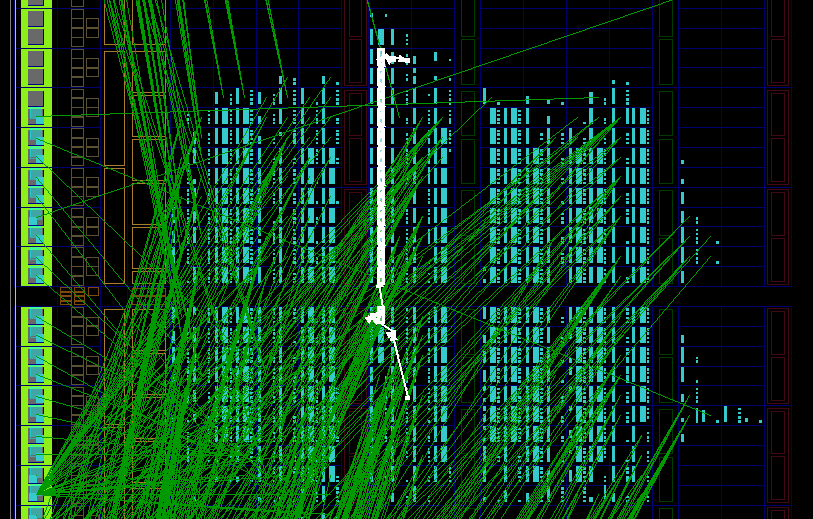
\includegraphics[width=0.9\textwidth]{./images/fig64_32_layout}
	\caption{\textit{Layout} de la implementación del algoritmo TEA de 64 bits de tamaño de palabra y 32 rondas de cifrado/descifrado.}
	\label{fig64_32_layout}
\end{figure}

\begin{figure}[H]
	\centering
	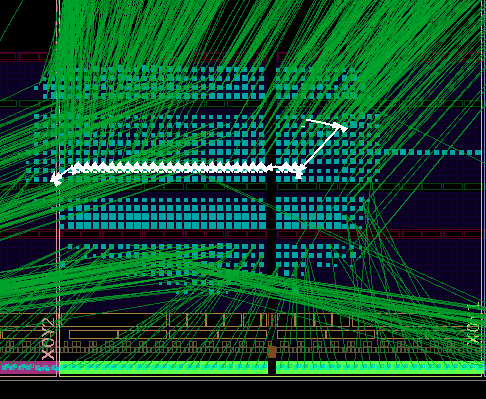
\includegraphics[width=0.9\textwidth]{./images/fig128_32_layout}
	\caption{\textit{Layout} de la implementación del algoritmo TEA de 128 bits de tamaño de palabra y 32 rondas de cifrado/descifrado.}
	\label{fig128_32_layout}
\end{figure}


En el caso de este algoritmo los parámetros que se variaron y cómo se variaron se muestran en la Tabla \ref{tabVariacionTEA} donde se fijó la cantidad de rondas en el valor nominal del algoritmo, 32 rondas de cifrado/descifrado\footnote{Para tamaños de palabra mayores a 128 se consideró innecesario el análisis debido a que ya un tamaño de palabra tan grande no es óptimo de utilizar bajo ninguna circunstancia.}.  Además en esa misma tabla se muestra el consumo de recursos del FPGA al variar esos parámetros. Note en los Listados \ref{lstCipherTEA} y \ref{lstDecipherTEA} como por el algoritmo no es posible variar independientemente el tamaño de la llave del tamaño de la palabra a cifrar y por tanto no es posible realizar un análisis independiente del análisis de la variación del tamaño de llave y como afecta los recursos del FPGA. 

% Table generated by Excel2LaTeX from sheet 'datos'
\begin{table}[htbp]
  \centering
  \caption{Variación de parámetros del algoritmo TEA y consumo de recursos del FPGA.}
    \begin{tabular}{rrrrrrr}
    \toprule
    \begin{tabular}[c]{@{}l@{}}Tamaño\\palabra\\(bits)\end{tabular}  & \begin{tabular}[c]{@{}l@{}}Tamaño\\llave\\(bits)\end{tabular} & \begin{tabular}[c]{@{}l@{}}LUT as\\Logic\end{tabular}  & Slice L & Slice M & \begin{tabular}[c]{@{}l@{}}Slice\\Registers\end{tabular} & \begin{tabular}[c]{@{}l@{}}Frecuencia \\máx. (MHz)\end{tabular}   \\
    \midrule
    8     & 32    & 217   & 45    & 27    & 176   & 434,783 \\
    16    & 64    & 383   & 74    & 38    & 328   & 392,157 \\
    32    & 128   & 737   & 133   & 90    & 632   & 338,983 \\
    64    & 256   & 1439  & 243   & 179   & 1240  & 303,030 \\
    128   & 512   & 2841  & 439   & 357   & 2456  & 217,391 \\

    \bottomrule
    \end{tabular}%
  \label{tabVariacionTEA}%
\end{table}%
		
De la Tabla \ref{tabVariacionTEA} se pueden extraer las gráficas que se muestran en las Figuras \ref{figSlicesTEA}, \ref{figSliceRegsLutsTEA} y \ref{figFrecuenciasTEA}.

La Figura \ref{figSlicesTEA} muestra como varía la cantidad de \textit{slices} tanto de tipo L como M conforme el tamaño de palabra varía. La Figura \ref{figSliceRegsLutsTEA} muestra como varía la cantidad de \textit{slice registers} y LUTs al variar el tamaño de la palabra. Note como después de variar la palabra de 32 bits a 64 bits la cantidad de recursos comienza a aumentar mostrando un comportamiento exponencial. Además la relación de ambas gráficas es la esperada ya que muestran la misma tendencia debido a que los \textit{slices} se encuentran compuestos por registros y LUTs.

\begin{figure}[H]
	\centering
	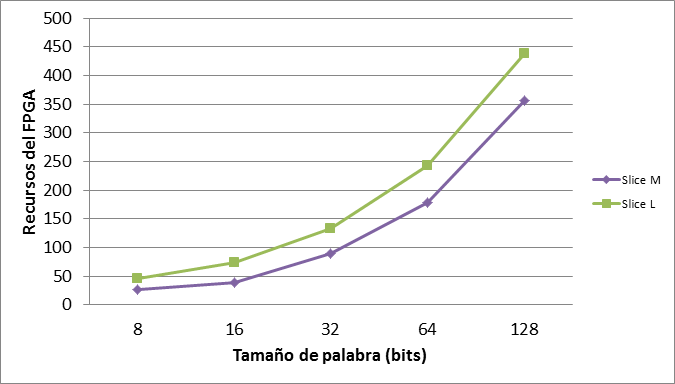
\includegraphics[width=0.9\textwidth]{./images/figSlicesTEA}
	\caption{Gráfica de variación de \textit{slice L} y \textit{slice M} contra la variación del tamaño de palabra en bits al implementar el algoritmo TEA.}
	\label{figSlicesTEA}
\end{figure}
\begin{figure}[H]
	\centering
	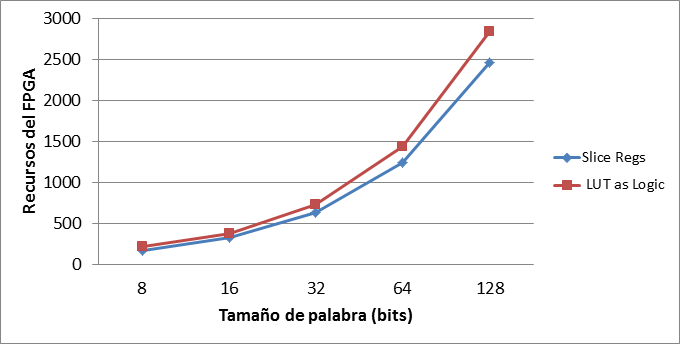
\includegraphics[width=0.9\textwidth]{./images/figSliceRegsLutsTEA}
	\caption{Gráfica de variación de \textit{slice registers} y LUTs contra la variación del tamaño de palabra en bits al implementar el algoritmo TEA.}
	\label{figSliceRegsLutsTEA}
\end{figure}

La Figura \ref{figFrecuenciasTEA} muestra la variación de la frecuencia máxima de reloj conforme el tamaño de palabra varía. El comportamiento es el esperado hasta cierto punto, ya que la frecuencia de reloj disminuye pero era esperado que la misma disminuyera de forma exponencial al igual que el consumo de recursos iba aumentando. Esto puede deberse a que la herramienta de desarrollo optimiza el proceso de \textit{place \& route} para lograr la mejor respuesta del diseño.

\begin{figure}[H]
	\centering
	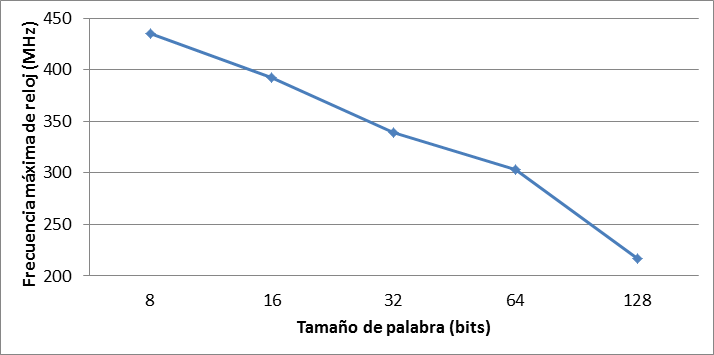
\includegraphics[width=0.9\textwidth]{./images/figFrecuenciasTEA}
	\caption{Gráfica de variación de la frecuencia máxima de reloj contra la variación del tamaño de palabra en bits al implementar el algoritmo TEA.}
	\label{figFrecuenciasTEA}
\end{figure}	
	
Finalmente los datos de la Tabla \ref{tabVariacionTEA} fueron normalizados respecto al valor mínimo de cada columna (por ejemplo 217 en la columna \textit{LUT as Logic}) con la finalidad de dar un análisis más acertado sobre cual sería el tamaño de palabra más conveniente a utilizar para este algoritmo. Los datos normalizados se muestran en la Tabla \ref{tabNormalizadoTEA} y se reflejan en la gráfica de la Figura \ref{figNormalizadoTEA}.

% Table generated by Excel2LaTeX from sheet 'datos'
\begin{table}[htbp]
  \centering
  \caption{Variación de parámetros del algoritmo TEA y consumo de recursos del FPGA normalizados.}
    \begin{tabular}{rrrrrrr}
    \toprule
    \begin{tabular}[c]{@{}l@{}}Tamaño\\palabra\\(bits)\end{tabular}  & \begin{tabular}[c]{@{}l@{}}Tamaño\\llave\\(bits)\end{tabular} & \begin{tabular}[c]{@{}l@{}}LUT as\\Logic\end{tabular}  & Slice L & Slice M & \begin{tabular}[c]{@{}l@{}}Slice\\Registers\end{tabular} & \begin{tabular}[c]{@{}l@{}}Frecuencia \\máx. reloj\end{tabular}   \\
    \midrule
    8     & 32    & 1,00  & 1,00  & 1,00  & 1,00  & 2,00 \\
    16    & 64    & 1,76  & 1,64  & 1,41  & 1,86  & 1,80 \\
    32    & 128   & 3,40  & 2,96  & 3,33  & 3,59  & 1,56 \\
    64    & 256   & 6,63  & 5,40  & 6,63  & 7,05  & 1,39 \\
    128   & 512   & 13,09 & 9,76  & 13,22 & 13,95 & 1,00 \\
    \bottomrule
    \end{tabular}%
  \label{tabNormalizadoTEA}%
\end{table}%

\begin{figure}[H]
	\centering
	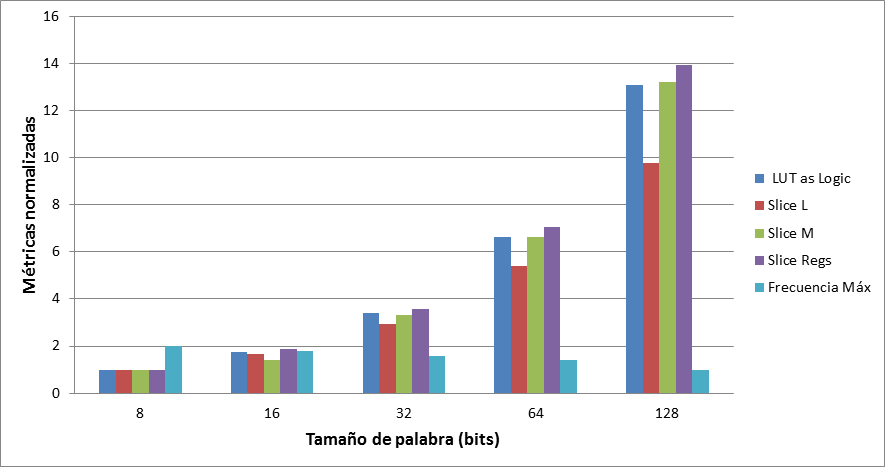
\includegraphics[width=1\textwidth]{./images/figNormalizadoTEA}
	\caption{Gráfica de consumo de recursos y frecuencia máxima (normalizados respecto al valor mínimo) del FPGA contra la variación del tamaño de palabra en bits al implementar el algoritmo TEA.}
	\label{figNormalizadoTEA}
\end{figure}
	
	
Note nuevamente como los recursos muestran el comportamiento exponencial descrito en las otras gráficas, pero como esta gráfica en particular los datos se muestran normalizados, el análisis se puede realizar de manera global.

Analizando la gráfica de la Figura \ref{figNormalizadoTEA} el comportamiento esperado es que al duplicar el tamaño de palabra se debe aumentar la cantidad de recursos consumidos en el FPGA al doble, así como reducir a la mitad la frecuencia máxima de reloj. Contrario a los resultados esperados se observa como conforme se varía el tamaño de palabra los recursos tienden ser menores al doble y la proporción se aleja cada vez más de ser el doble. Esto se puede deber nuevamente a la herramienta de desarrollo que puede optimizar el diseño \textcolor{red}{DE QUE MANERA??????????}. En el caso de la frecuencia máxima de reloj se observa como hasta que la palabra llega a ser de 128 bits se obtiene la frecuencia de la mitad de la frecuencia para el tamaño de palabra de 8 bits, esto se debe nuevamente (y como se explicó anteriormente en el análisis de la Figura \ref{figFrecuenciasTEA}) a la herramienta de desarrollo.


Finalmente bajo los análisis dados anteriormente se puede concluir que el tamaño de palabra ideal podría ser cualquiera menor a 32 bits. Las razones de esto son las siguientes:

\begin{itemize}
\item El tamaño de palabra de 32 bits, implica una entrada de texto plano de 64 bits, la cual se ajusta perfectamente al tamaño de palabra actual de la mayoría de procesadores de computadoras personales. También existen muchos microcontroladores con procesadores con tamaños de palabra de 32 bits o 16 bits, lo cual indicaría para el algoritmo tamaños de palabra de 8 bits o 16 bits. El beneficio de ``acoplar'' de alguna manera las entradas y salidas del algoritmo a las entradas y salidas del procesador es que en el cifrado puede procesar inmediatamente la información conforme esta sale del procesador y en el caso del descifrado es que puede entregar inmediamente al procesador la información descifrada y continuar descifrando datos.\footnote{Inclusive existen microcontroladores con procesadores de 8 bits por ejemplo el HC 08 de Freescale (\url{http://www.freescale.com/products/more-processors/8-bit-mcus/hc08:HC08FAMILY?cof=0&am=0}). Entonces sería válido realizar un análisis para 4 bits de tamaño de palabra del algoritmo.}

\item Las frecuencias máximas de reloj a las que trabajan esas implementaciones son mucho mayores que en las implementaciones de palabras de mayor tamaño.

\item Aunque puede ocurrir una disminución en el nivel de seguridad del algoritmo al trabajar con palabras más pequeñas, esta se puede aumentar aumentando la cantidad de rondas de cifrado y al trabajar a una frecuencia más alta el impacto en el desempeño no es tanto.

\item Se ahorra una gran cantidad de recursos en el FPGA el cual se traduce directamente en costos de producción.
\end{itemize}

\clearpage
\section{Resultados y análisis del algoritmo RC5}
Inicialmente se corroboró que el algoritmo funcionara correctamente, esto se logró comparando los resultados de texto cifrado y descifrado con el código en C que se encuentra en el artículo del algoritmo \citep{rivest}. La Tabla \ref{tabSimRC51} muestra el resultado de cifrado y descifrado al simular variando el tamaño de palabra y la Tabla \ref{tabSimRC52} muestra los resultados de simular variando el tamaño de llave. Al igual que el algoritmo anterior la tabla en la columna \textit{layout} indica un número de figura al cual está ligado la implementación.

\begin{table}[htbp]
  \centering
  \caption{Resultados de simulación para distintos tipos del RC5 variando el tamaño de palabra con una llave de 16 bytes igual a 91CEA91001A5556351B241BE19465F91$_{hex}$.}
    \begin{tabular}{lrrr}
    \toprule
	\begin{tabular}[c]{@{}l@{}}Tipo\\RC5 \end{tabular} & Texto plano (hex) & Texto cifrado (hex) & Figura \textit{layout} \\
    \midrule
	16/12/16 & a5214b15 & a496d848 & \ref{fig16_12_16_layout} \\
	\midrule
	32/12/16 & \begin{tabular}[c]{@{}l@{}}eedba521\\6d8f4b15\end{tabular} & \begin{tabular}[c]{@{}l@{}}ac13c0f7\\52892b5b\end{tabular} & \ref{fig32_12_16_layout}\\
	\midrule
	64/12/16 & \begin{tabular}[c]{@{}l@{}}00000000\\eedba521\\00000000\\6d8f4b15\end{tabular} & \begin{tabular}[c]{@{}l@{}}829c9641\\f96ead46\\f91c9890\\738c8807\end{tabular} & \ref{fig64_12_16_layout}\\
    \bottomrule
    \end{tabular}%
  \label{tabSimRC51}%
\end{table}%


\begin{table}[htbp]
  \centering
  \caption{Resultados de simulación para distintos tipos del RC5 variando el tamaño de llave.}
    \begin{tabular}{lrrrr}
    \toprule
    \begin{tabular}[c]{@{}l@{}}Tipo\\RC5 \end{tabular} & Llave (hex) & Texto plano (hex) & Texto cifrado (hex) & \begin{tabular}[c]{@{}l@{}}Figura\\\textit{layout}\end{tabular}\\
    \midrule
32/16/7 & \begin{tabular}[c]{@{}l@{}}2c5b2aa\\c54b1a5\end{tabular} & \begin{tabular}[c]{@{}l@{}}12153524\\c0895e81\end{tabular} & \begin{tabular}[c]{@{}l@{}}9e6edba6\\9b789a70\end{tabular} & \ref{fig32_16_7_layout} \\
\midrule
32/16/12 & \begin{tabular}[c]{@{}l@{}}5e68d4\\564a2c\\5b2aac\\54b1a5\end{tabular} & \begin{tabular}[c]{@{}l@{}}f232b52\\aeeebba13\end{tabular} & \begin{tabular}[c]{@{}l@{}}a4db4976\\94726be1\end{tabular} & \ref{fig32_16_12_layout} \\
\midrule
32/16/16 & \begin{tabular}[c]{@{}l@{}}d4543e13\\5e68d456\\4a2c5b2a\\ac54b1a5\end{tabular} & \begin{tabular}[c]{@{}l@{}}eedba521\\6d8f4b15\end{tabular} & \begin{tabular}[c]{@{}l@{}}b6c95c5c\\e51616b8\end{tabular} & \ref{fig32_16_16_layout} \\
    \bottomrule
    \end{tabular}%
  \label{tabSimRC52}%
\end{table}%


\begin{figure}
	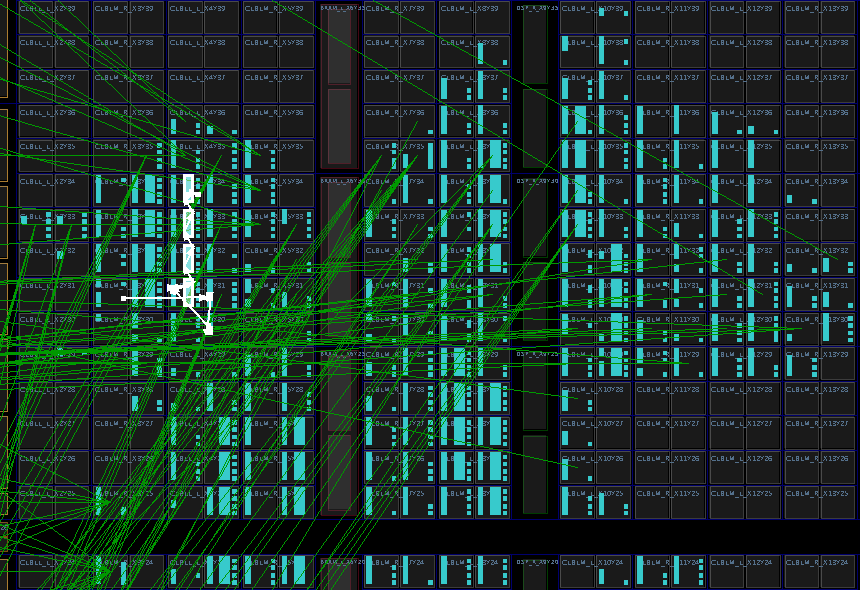
\includegraphics[width=0.9\textwidth]{./images/fig16_12_16_layout}
	\caption{\textit{Layout} de la implementación del algoritmo RC5-16/12/16.}
	\label{fig16_12_16_layout}
\end{figure}

\begin{figure}
	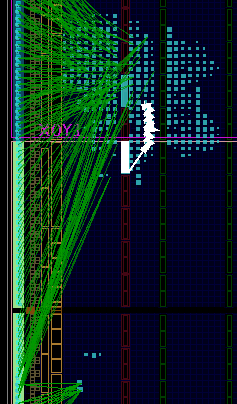
\includegraphics[width=0.9\textwidth]{./images/fig32_12_16_layout}
	\caption{\textit{Layout} de la implementación del algoritmo RC5-32/12/16.}
	\label{fig32_12_16_layout}
\end{figure}

\begin{figure}
	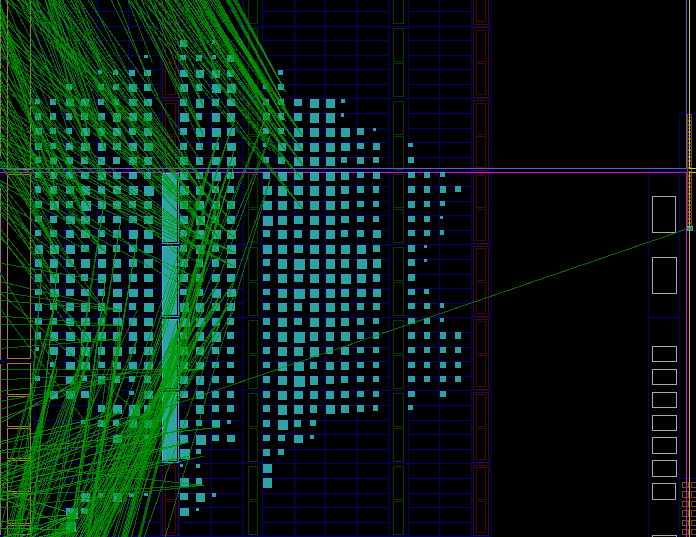
\includegraphics[width=0.9\textwidth]{./images/fig64_12_16_layout}
	\caption{\textit{Layout} de la implementación del algoritmo RC5-64/12/16.}
	\label{fig64_12_16_layout}
\end{figure}
%%%%%%%%%%%%%%%%%%%%%%%%%%%%%%%%%%
\begin{figure}[H]
	\centering
	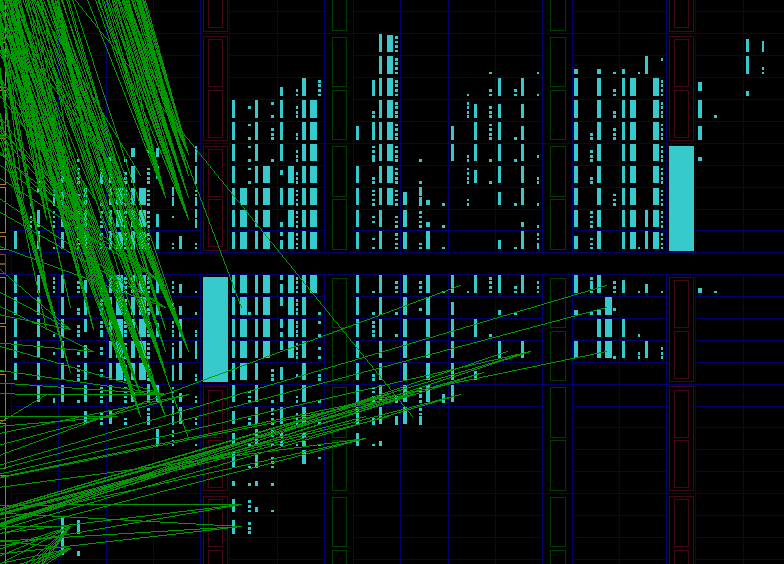
\includegraphics[width=0.85\textwidth]{./images/fig32_16_7_layout}
	\caption{\textit{Layout} de la implementación del algoritmo RC5-32/16/7.}
	\label{fig32_16_7_layout}
\end{figure}

\begin{figure}
	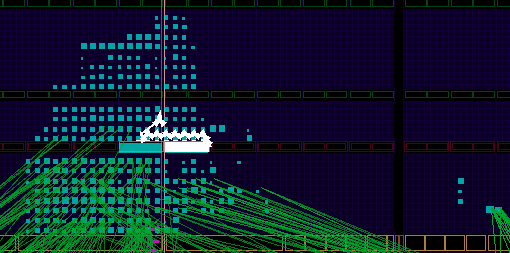
\includegraphics[width=1\textwidth]{./images/fig32_16_12_layout}
	\caption{\textit{Layout} de la implementación del algoritmo RC5-32/16/12.}
	\label{fig32_16_12_layout}
\end{figure}


\begin{figure}
	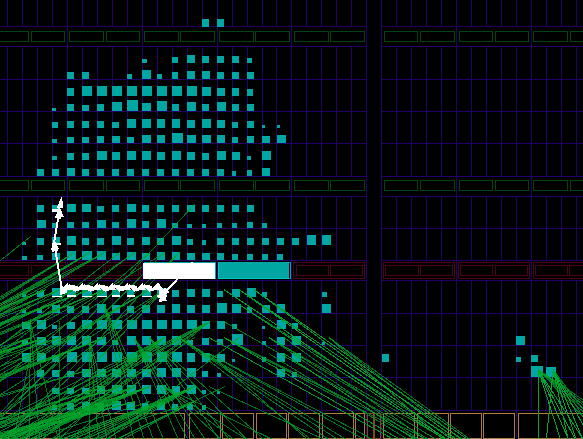
\includegraphics[width=0.9\textwidth]{./images/fig32_16_16_layout}
	\caption{\textit{Layout} de la implementación del algoritmo RC5-32/16/16.}
	\label{fig32_16_16_layout}
\end{figure}

Posterior a verificar el funcionamiento del algoritmo mediante se procedió a sintetizar e implementar el algoritmo (con las variaciones descritas en las Tablas \ref{tabSimRC51} y \ref{tabSimRC52}) haciendo uso del \textit{Vivado Design Suite}. Con esto se obtuvo la variación de recursos del FPGA mostrada en las Tablas \ref{tabVariacionRC5llave} y \ref{tabVariacionRC5palabra} mediante el mismo procedimiento descrito en la Sección \ref{resultadosAnalisisTEA}. En el caso de las variaciones de palabra se realizó de esta manera porque el autor del algoritmo indica que la implementación nominal del algoritmo es la RC5-32/12/16  y por tanto se quería observar la variación en el consumo de recursos alrededor del tamaño de palabra nominal, ajustandose a valores típicos de tamaños de palabra (potencias de 2). En el caso del tamaño de llave la variación se llevó a cabo de esta manera para poder realizar el análisis comparativo más adelante.

\begin{table}[htbp]
  \centering
    \begin{tabular}{rrrrrrrr}
    \toprule
    \begin{tabular}[c]{@{}l@{}}Tamaño\\llave\\(bytes)\end{tabular} & \begin{tabular}[c]{@{}l@{}}LUT as\\Logic\end{tabular} & RAM   & \begin{tabular}[c]{@{}l@{}}LUT as\\Memory\end{tabular} & Slice L & Slice M & \begin{tabular}[c]{@{}l@{}}Slice\\Regs\end{tabular} & \begin{tabular}[c]{@{}l@{}}Frec.\\máx.\\(MHz)\end{tabular} \\
    \midrule
    7    & 993   & 2     & 8     & 180   & 135   & 685   & 227,27 \\
    12    & 993   & 2     & 8     & 194   & 127   & 688   & 217,39 \\
    16    & 991   & 2     & 8     & 187   & 129   & 688   & 212,77 \\
    \bottomrule
    \end{tabular}%
  \caption{Variación del tamaño de la llave y recursos del FPGA para el algoritmo RC5-32/16/B}
  \label{tabVariacionRC5llave}%
\end{table}%

\begin{table}[htbp]
  \centering
    \begin{tabular}{rrrrrrrr}
    \toprule
    \begin{tabular}[c]{@{}l@{}}Tamaño\\palabra\\(bits)\end{tabular} & \begin{tabular}[c]{@{}l@{}}LUT\\as Logic\end{tabular} & RAM   & \begin{tabular}[c]{@{}l@{}}LUT as\\Memory\end{tabular} & Slice L & Slice M & \begin{tabular}[c]{@{}l@{}}Slice\\Regs\end{tabular} & \begin{tabular}[c]{@{}l@{}}Frec.\\máx.\\(MHz)\end{tabular} \\
   \midrule
    16    & 578   & 0     & 40    & 112   & 82    & 446   & 377,36 \\
    32    & 972   & 2     & 8     & 188   & 139   & 687   & 212,77 \\
    64    & 1911  & 4     & 8     & 314   & 236   & 1273  & 192,31 \\
    \bottomrule
    \end{tabular}%
  \caption{Variación del tamaño de la palabra y recursos del FPGA para el algoritmo RC5-W/12/16}
  \label{tabVariacionRC5palabra}%
\end{table}%

\subsection{Resultados y análisis de la variación del tamaño de la llave}

De la Tabla \ref{tabVariacionRC5llave} se generó la gráfica mostrada en la Figura \ref{figllaveRC5}. La gráfica muestra la viaración del consumo de recursos del FPGA y la frecuencia máxima de reloj conforme varia el tamaño de llave, el comportamiento mostrado fue casi constante demostrando que la variación del tamaño de la llave de un tamaño mayor al doble no afecta el consumo de recursos del FPGA. Esto es muy valioso debido a que al aumentar el tamaño de llave se aumenta la seguridad del algoritmo pero no afecta el consumo de recursos del FPGA. En el aspecto que si afecta esta variación es en la cantidad de tiempo de procesamiento, ya que se debe leer y escribir más veces a la memoria que resguarda la llave. Así se podría concluir del análisis que el tamaño de llave ideal depende de cuanta seguridad se quiere y que tan rápido se necesita llevar a cabo el proceso de cifrado/descifrado de los datos.

\begin{figure}[H]
	\centering
	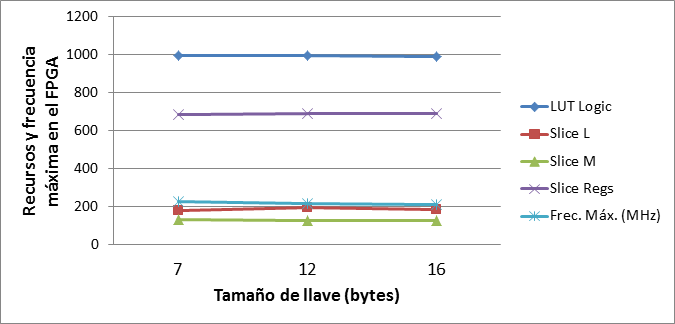
\includegraphics[width=0.8\textwidth]{./images/figLlaveRC5}
	\caption{Gráfica de consumo de recursos y frecuencia máxima del FPGA contra la variación del tamaño de llave en bytes al implementar el algoritmo RC5.}
	\label{figllaveRC5}
\end{figure}


\subsection{Resultados y análisis de la variación del tamaño de la palabra}
De la Tabla \ref{tabVariacionRC5palabra} se extrajeron las gráficas de la Figuras \ref{figSlicesRC5}, \ref{figSliceRegsLutsRC5}, \ref{figRamRC5} y \ref{figFrecuenciasRC5}. 

La Figura \ref{figSlicesRC5} muestra la variación de la cantidad de \textit{Slices L} y \textit{Slices M} consumidos conforme se varía el tamaño de palabra. Además la Figura \ref{figSliceRegsLutsRC5} muestra la variación de la cantidad de \textit{Slice Registers} y LUTs variando el tamaño de palabra. Como se puede observar de ambas figuras los datos muestran un comportamiento exponencial y similar, esto se debe a que, como se mencionó en el análisis del algoritmo TEA, los \textit{Slices} se componen de registros y LUTs.


\begin{figure}[H]
	\centering
	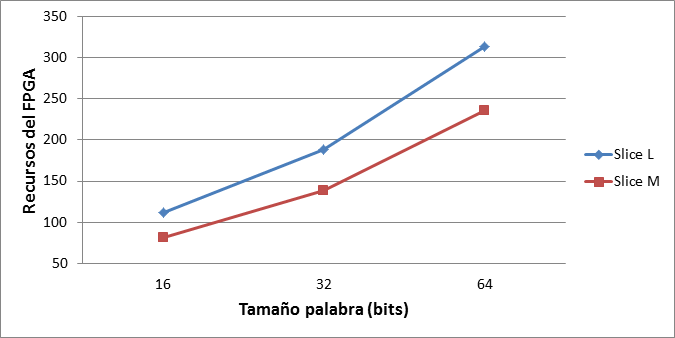
\includegraphics[width=0.8\textwidth]{./images/figSlicesRC5}
	\caption{Gráfica de consumo de \textit{Slices L} y \textit{Slices M} del FPGA contra la variación del tamaño de la palabra al implementar el algoritmo RC5.}
	\label{figSlicesRC5}
\end{figure}

\begin{figure}[H]
	\centering
	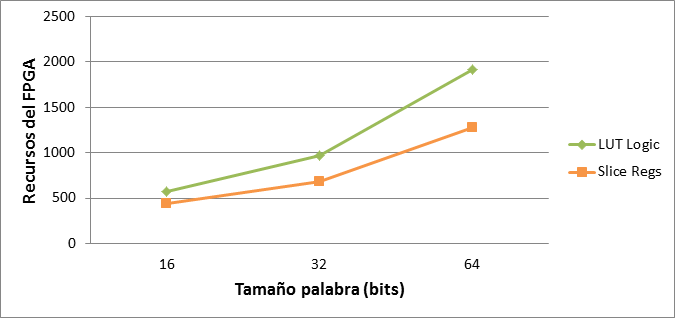
\includegraphics[width=0.8\textwidth]{./images/figSliceRegsLutsRC5}
	\caption{Gráfica de consumo de \textit{Slice Registers} y LUTs del FPGA contra la variación del tamaño de la palabra al implementar el algoritmo RC5.}
	\label{figSliceRegsLutsRC5}
\end{figure}

La Figura \ref{figRamRC5} muestra el consumo de \textit{LUT as memory} y bloques de memoria RAM al variar el tamaño de palabra. Como se puede observar, la implementación del algoritmo con tamaño de palabra de 16 bits no hace uso de ningún RAM y más bien utiliza LUTs como memoria. Posteriormente las otras dos implementaciones hacen uso de RAMs causando el desuso de gran parte de los LUTs utilizados como memoria, disminuyendo esta métrica de manera drástica y manteniéndola constante. Finalmente de la gráfica se puede observar el comportamiento lineal del consumo de bloques de memoria RAM ajustándose a lo esperado de que al duplicar el tamaño de palabra se duplique el uso de bloques de memoria RAM.
\begin{figure}[H]
	\centering
	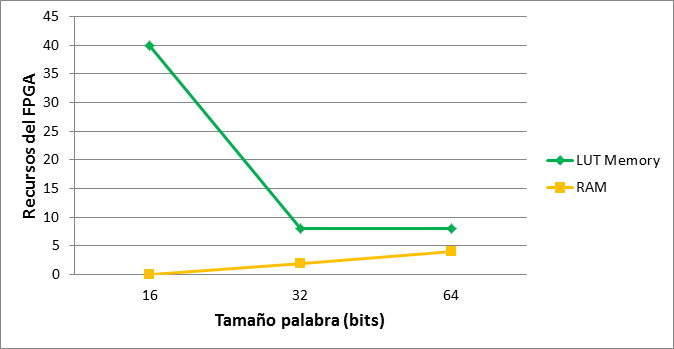
\includegraphics[width=0.8\textwidth]{./images/figRamRC5}
	\caption{Gráfica de consumo de \textit{LUT as memory} y bloques de memoria RAM del FPGA contra la variación del tamaño de la palabra al implementar el algoritmo RC5.}
	\label{figRamRC5}
\end{figure}

La Figura \ref{figFrecuenciasRC5} muestra la variación de la frecuencia máxima de reloj al variar el tamaño de palabra. Como se puede observar para la implementación de tamaño de palabra de 16 bits la frecuencia es mucho más alta que para las otras dos implementaciones. Esto se debe al cambio de utilizar LUTs como memoria a bloques de memoria RAM, los cuales son mucho más lentos. Además note como al pasar de 32 bits de tamaño de palabra a 64 bits, la variación de frecuencia máxima es pequeña, debido a que al no mapear la memoria a LUTs sino a bloques de memoria RAM no se tiene una memoria distribuida sino centralizada produciendo que la frecuencia sea mucho más estable.
\begin{figure}[H]
	\centering
	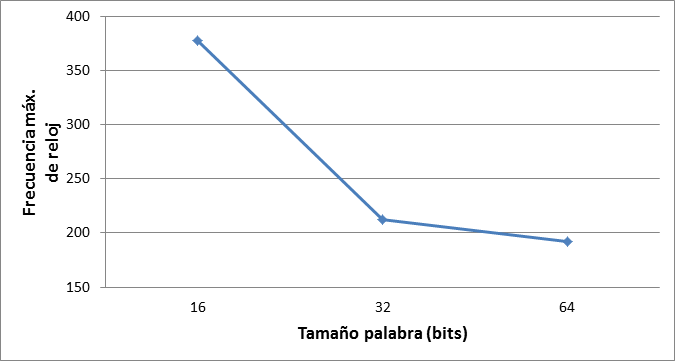
\includegraphics[width=0.8\textwidth]{./images/figFrecuenciasRC5}
	\caption{Gráfica de frecuencia máxima del FPGA contra la variación del tamaño de la palabra al implementar el algoritmo RC5.}
	\label{figFrecuenciasRC5}
\end{figure}

Finalmente y al igual que con el algoritmo TEA se normalizaron los datos para tener una visión global para analizar. Los datos normalizados se muestran en la Tabla \ref{tabNormalizadoRC5} y se reflejan en la Figura \ref{figNormalizadoRC5}. Se exceptúo del análisis normalizado las métricas \textit{LUT as memory} y RAM debido a que RAM no era un parámetro normalizable (para el tamaño de palabra de 16 bits es cero) y que \textit{LUT as memory} varió de forma inconsistente por el uso de bloques de memoria RAM, agregando poco valor al análisis. De la gráfica se observa VOY A AGUANTARLA A HABLAR CON EL PROFE PORQUE LA GRAFICA SE COMPORTA IGUAL A LA DEL TEA.

\begin{table}[htbp]
  \centering
    \begin{tabular}{rrrrrr}
    \toprule
    \begin{tabular}[c]{@{}l@{}}Tamaño\\palabra\\(bits)\end{tabular} & \begin{tabular}[c]{@{}l@{}}LUT\\as Logic\end{tabular} &   Slice L & Slice M & \begin{tabular}[c]{@{}l@{}}Slice\\Regs\end{tabular} & \begin{tabular}[c]{@{}l@{}}Frec.\\máx.\\(MHz)\end{tabular} \\
   \midrule
    16    & 1     & 1     & 1     & 1     & 1,96 \\
    32    & 1,68  & 1,68  & 1,70  & 1,54  & 1,11 \\
    64    & 3,31  & 2,80  & 2,88  & 2,85  & 1 \\
    \bottomrule
    \end{tabular}%
  \caption{Variación del tamaño de la palabra y recursos del FPGA normalizados para el algoritmo RC5-W/12/16.}
  \label{tabNormalizadoRC5}%
\end{table}%

\begin{figure}[H]
	\centering
	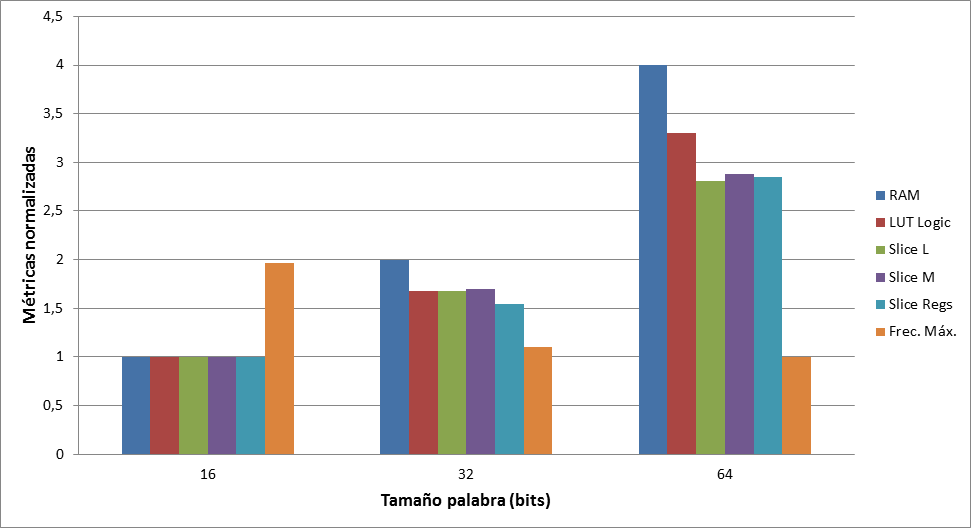
\includegraphics[width=1\textwidth]{./images/figNormalizadoRC5}
	\caption{Gráfica de consumo de recursos y frecuencia máxima (normalizados respecto al valor mínimo) del FPGA contra la variación del tamaño de palabra al implementar el algoritmo RC5.}
	\label{figNormalizadoRC5}
\end{figure}


\clearpage
\section{Análisis comparativo}
Para realizar el análisis comparativo es necesario tener un punto de referencia para la escogencia de los parámetros de cada algoritmo con el fin de lograr un análisis justo. Esto se logró tomando como referencia lo descrito en los artículos que describen cada algoritmo. En ambos artículos se hace una referencia a cual implementación del algoritmo es ``equivalente'' a utilizar el algoritmo DES. Citando ambos artículos:
\cite{rivest}
    \emph{``As an example, consider the problem of replacing DES with an "equivalent" RC5 algorithm. One might reasonable choose RC5-32/16/7 as such a replacement.''}

\cite{tea}
   \emph{``This type of algorithm can replace DES in software, and is short enough to write into almost any program on any computer.''}
 
Por tanto el RC5-32/16/7 y el TEA con 32 rondas y tamaño de palabra de 32 bits fueron elegidos para realizar el análisis comparativo.